%************************************************
\chapter{Case Study}\label{ch:case_study}
%************************************************
In order to evaluate the proposed solution in an empirical manner, the developed solution was deployed at an industrial company. This is a Smart Buildings company, which runs their services in a private Cloud deployment. The company offers products to monitor the users electricity and gas consumption in real-time. This leads to an increase in building-users awareness by providing real-time feedback through public dashboards \cite{sb}. A brief overview of their architecture is described in \autoref{sec:sb-architecture}. This company perfectly meets the requirements for evaluating the developed solution, because it is a relatively large system with load. Additionally, the solution was deemed to be useful for them, as they are currently missing insights into their performance. The process of deploying this system has been described in \autoref{sec:sb-process}. The results are described in \autoref{sec:sb-results}. Furthermore, the limitation of the case study is  described in \autoref{sec:sb-limitation}. At the end, an interview has been performed. The purpose of the interview with stakeholders is to collect data with respect to their perception of the solution. This interview is described in \autoref{sec:sb-interview}.

\section{Architecture} \label{sec:sb-architecture}
In order to serve their customers, the company has allocated a physical server consisting of $40$ cores and $128$ GB of RAM. Additionally, they have $900$ GB of storage data. This host machine is divided into six virtual machines. The six virtual machines work together as one system. Each virtual machine is responsible for running a number of services. These services can be found in \autoref{fig:sb-architecture}. In order to simplify the deployment, the employees of the company decided to assign a name to every VM\footnote{Note that the names are pseudo anonymized to not reveal valuable company details.}. The hosts are also presented in the architecture diagram. A small overview of the number of CPU, RAM and memory per VM can be found in \autoref{tab:vms}. As described in \autoref{sec:architecture}, the architecture consists of a single root-node, two super-nodes and four normal nodes. The structure can be found in \autoref{fig:sb-tree}. From this figure it becomes clear that host $0$ consumes two roles. Both as a root, and as a supernode.


\begin{figure}
    \centering
    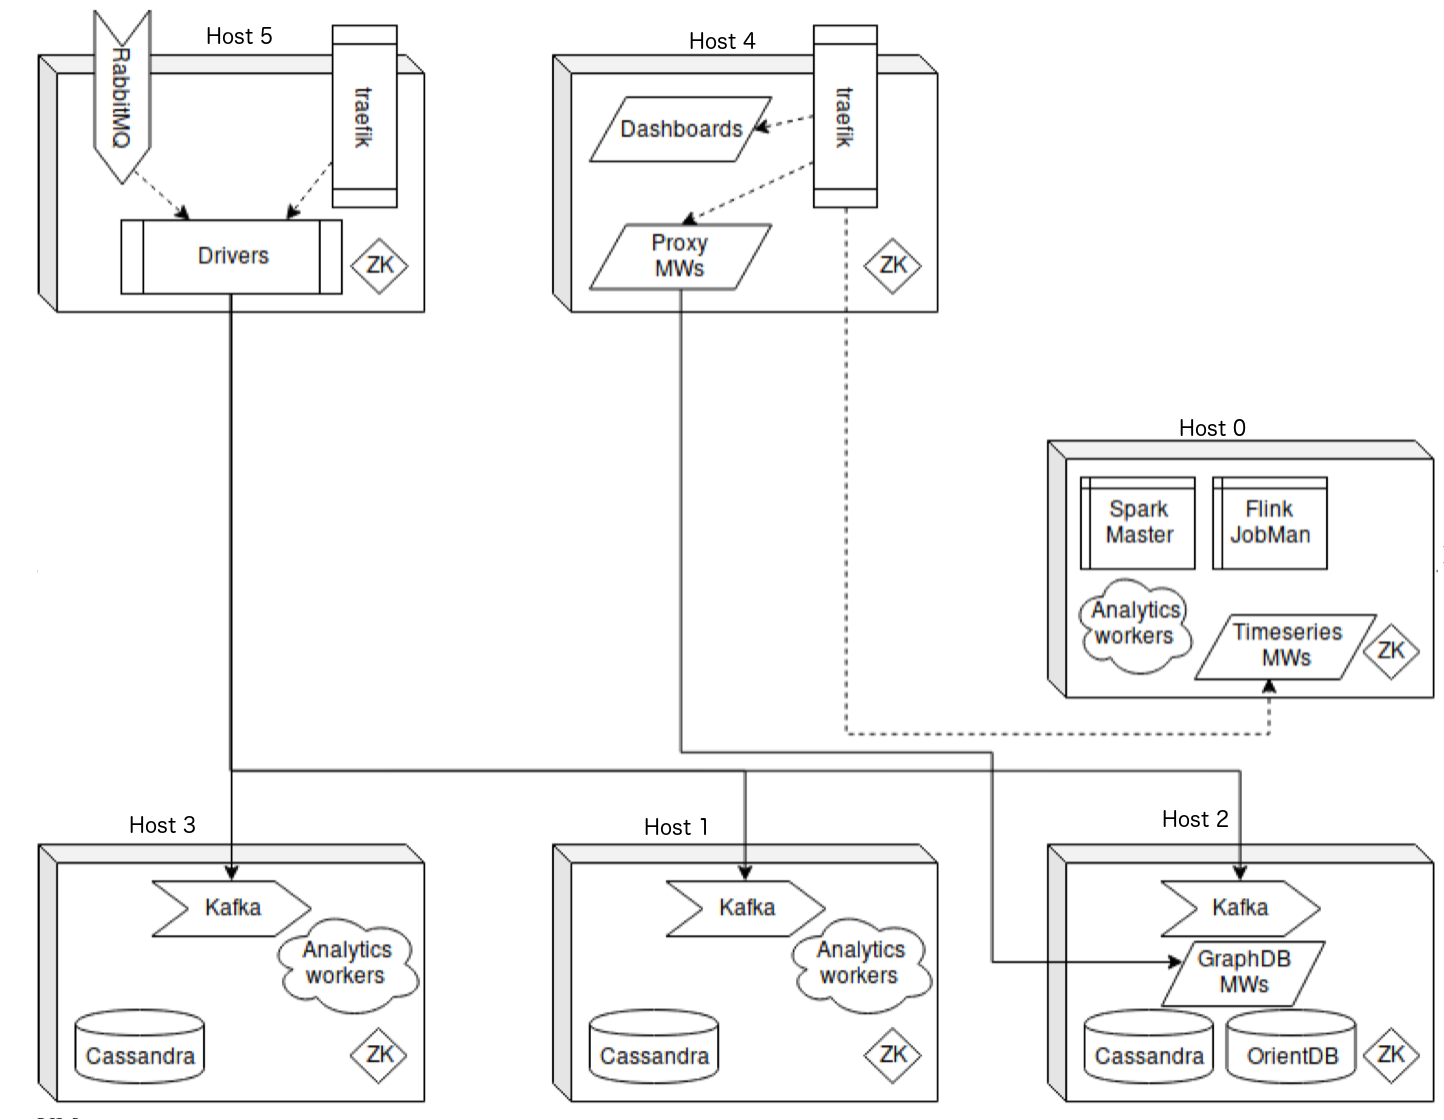
\includegraphics[width=\textwidth]{gfx/sb-architecture1.png}
    \caption{Smart Buildings architecture}
    \label{fig:sb-architecture}
\end{figure}

\begin{table}
    \centering
    \begin{tabular}{l|lrrr}
        Virtual Machine &IP & Cores & RAM & Memory \\ \hline
        Host $0$ & $192.168.1.13$ &$8$ & $16$ GB & $100$ GB \\
        Host $1$ & $192.168.1.11$ &$8$ & $16$ GB & $100$ GB \\
        Host $2$ & $192.168.1.12$ &$8$ & $16$ GB & $100$ GB \\
        Host $3$ & $192.168.1.10$ &$8$ & $16$ GB & $100$ GB \\
        Host $4$ & $192.168.1.14$ &$4$ & $8$ GB & $20$ GB \\
        Host $5$ & $192.168.1.15$ &$4$ & $8$ GB & $20$ GB \\
    \end{tabular}
    \caption{Overview of the architecture}
    \label{tab:vms}
\end{table}

\begin{figure}
    \centering
    \begin{forest}
        for tree={
            grow=south,
            rectangle, draw, minimum size=3ex, inner sep=1pt,s sep=7mm
        }
        [~~Root: Host $0$~~~ 
        [~~Supernode: Host $1$~~~ 
          [~~Node: Host $2$~~~]
          [~~Node: Host $3$~~~]
        ]
        [~~Supernode: Host $0$~~~
          [~~Node: Host $4$~~~]
          [~~Node: Host $5$~~~]
        ]
        ]
    \end{forest}
    \caption{Hierarchical overview of the Case study}
    \label{fig:sb-tree}
\end{figure}

\section{Deployment process} \label{sec:sb-process}
This section describes the process of deploying the implemented system on their architecture. This deployment has been made possible within several meetings throughout the Summer of 2019. They are shortly described in the subsections below. Each meeting last around three hours.

\subsection{First meeting}
During the first meeting, several issues showed up. Initially, the developed system was implemented in such a way that the nodes were communicating over their public IP address. However, it turned out that not every node was publicly accessible. More specifically, the program was updated, such that they communicate over their internal IP. Another issue was due to the amount of load going in and out their system. Therefore, the part of the program that monitors the network traffic with respect to the containers raised its CPU to above 100\% as can be seen in \autoref{fig:100}. After a short discussion, we decided to not deploy the program any more, and first solve the issues that showed up.

\begin{figure}
    \centering
    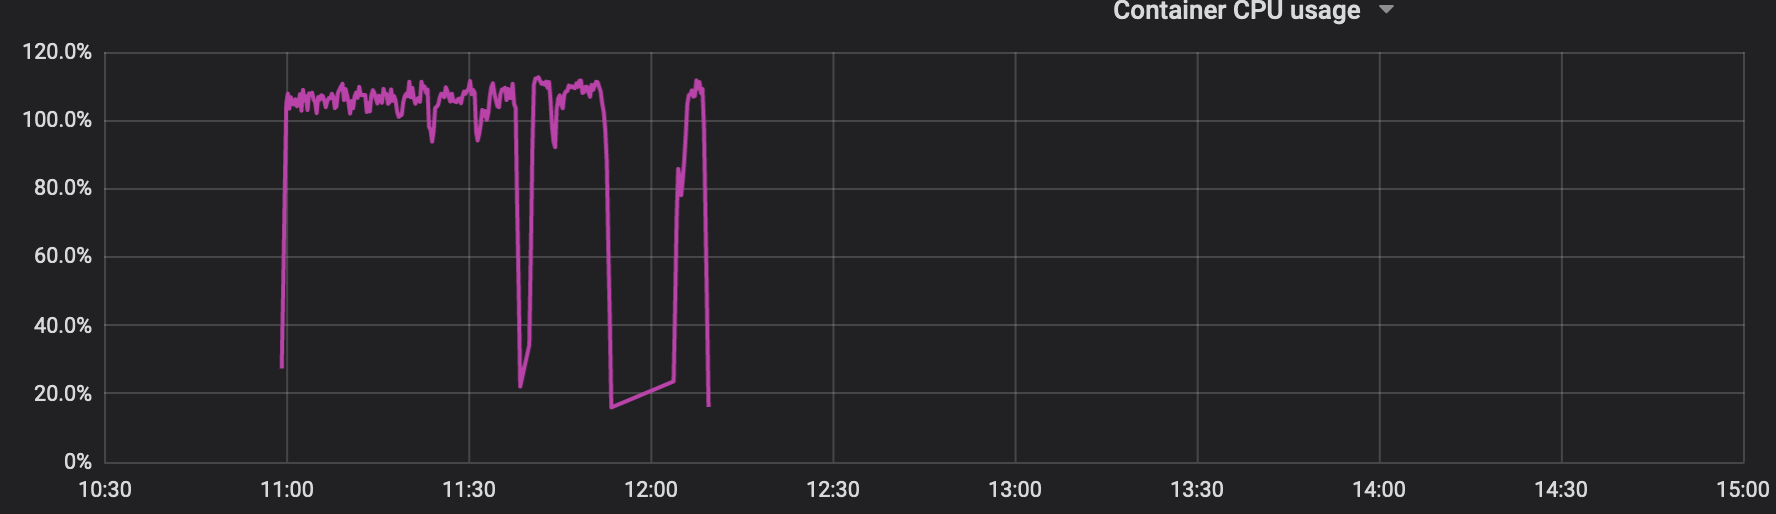
\includegraphics[width=\textwidth]{gfx/load-100.png}
    \caption{CPU data of the deployed system during the first meeting}
    \label{fig:100}
\end{figure}

\subsection{Second meeting}
In order to solve the issue described in the previous subsection, a sub sampling of the network monitoring was applied, as discussed in \autoref{sec:identify-traffic}. Therefore, instead of capturing all packets, the packets where captured for $x$ seconds, while sleeping $K*x$ seconds. However, for every packet that is coming from a peer within the system, the program tries to assign this packet directly to a remote Docker container. Therefore, there was still a significant amount of communication overhead, which can be seen in \autoref{fig:60}. Eventually, the program kept growing CPU resources consumed, which lead to the conclusion that the program was not efficient enough. Therefore, the program was not deployed during this meeting.

\begin{figure}[H]
    \centering
    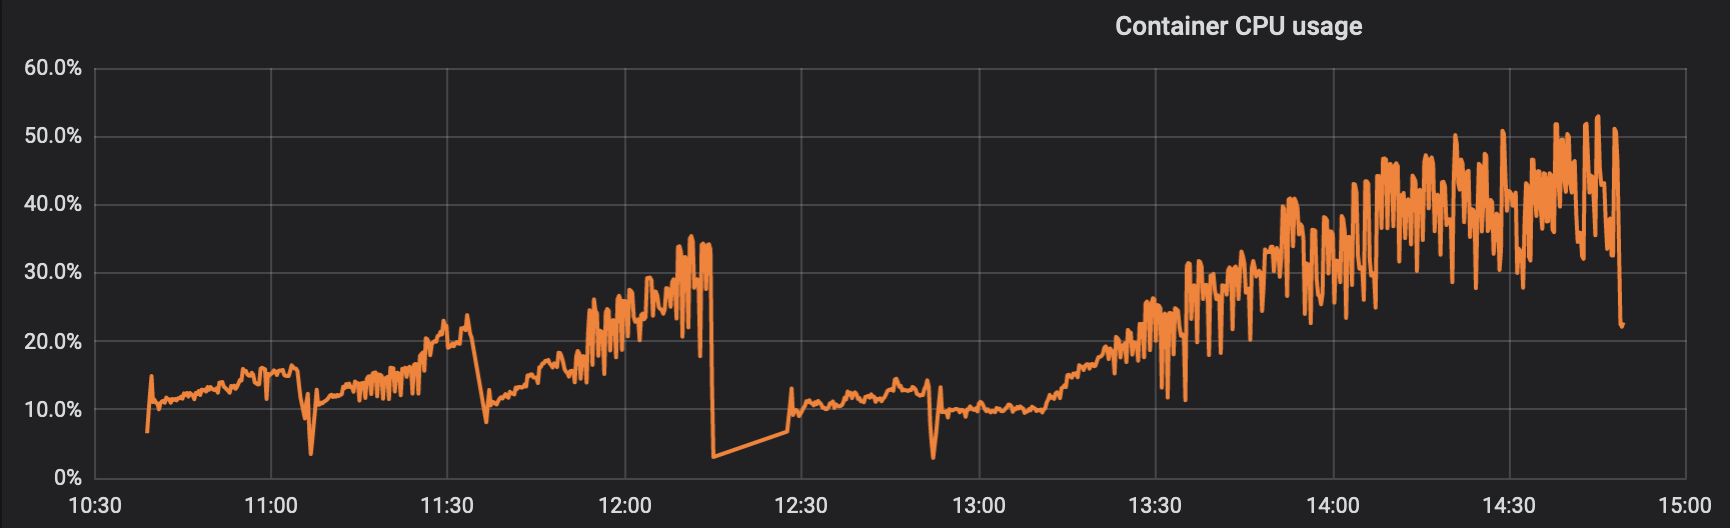
\includegraphics[width=\textwidth]{gfx/load-60.png}
    \caption{CPU data of the deployed system during the second meeting}
    \label{fig:60}
\end{figure}

\begin{figure}[H]
    \subfloat[Host $3$]{%
        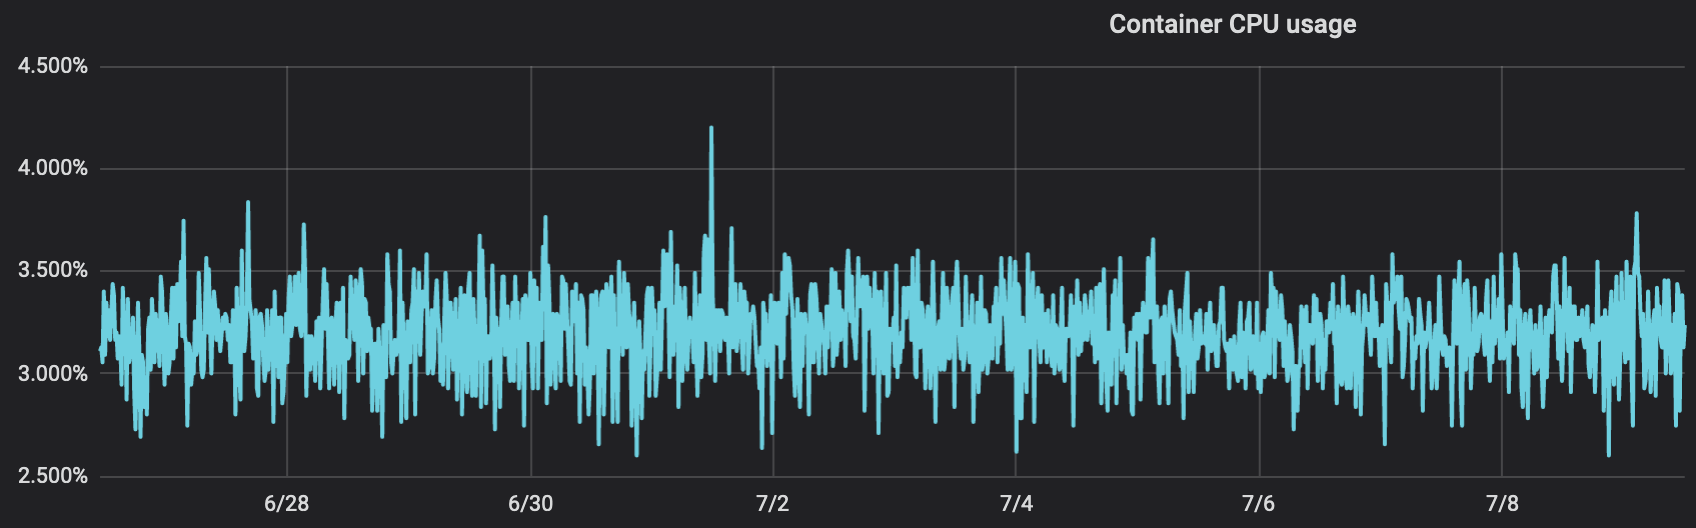
\includegraphics[width=0.45\textwidth]{gfx/asgard.png}
        \label{fig:deployment:asgard}
    }\qquad
    \subfloat[Host $4$]{
        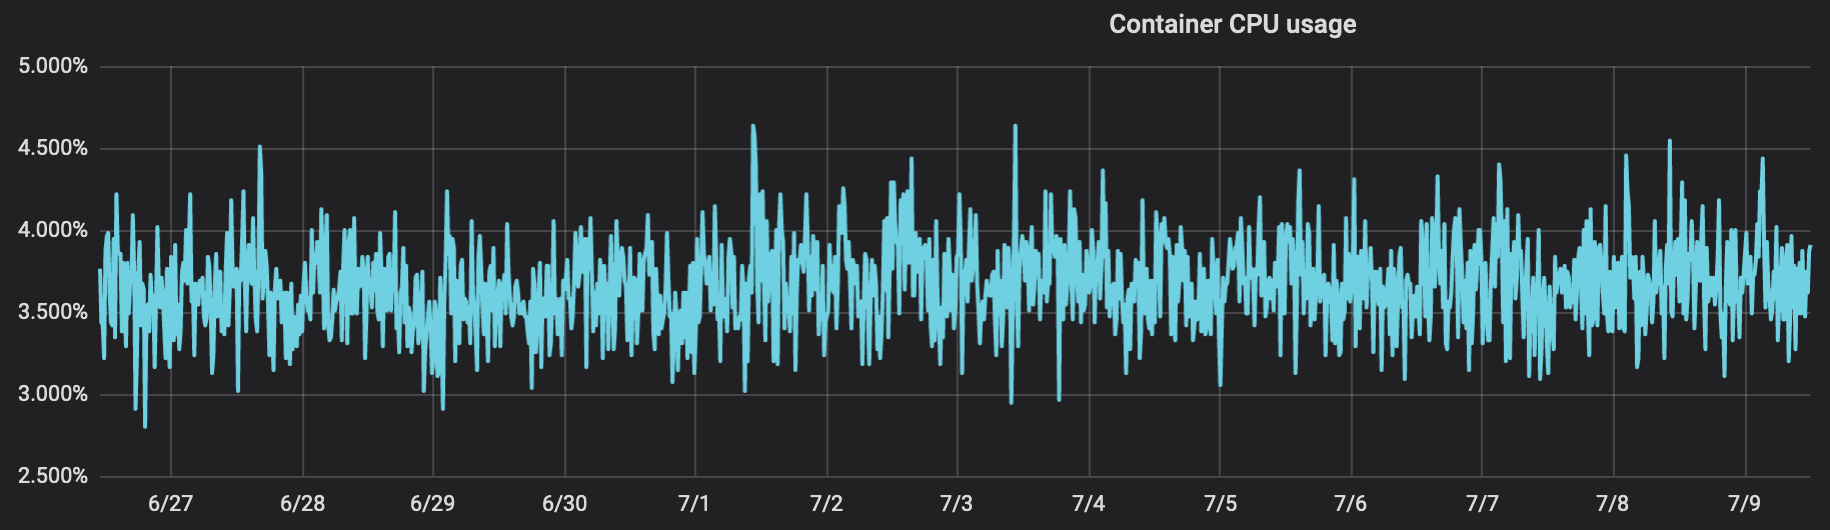
\includegraphics[width=0.45\textwidth]{gfx/midgard.png}%
        \label{fig:deployment:midgard}
    }
    
    \subfloat[Host $1$]{%
        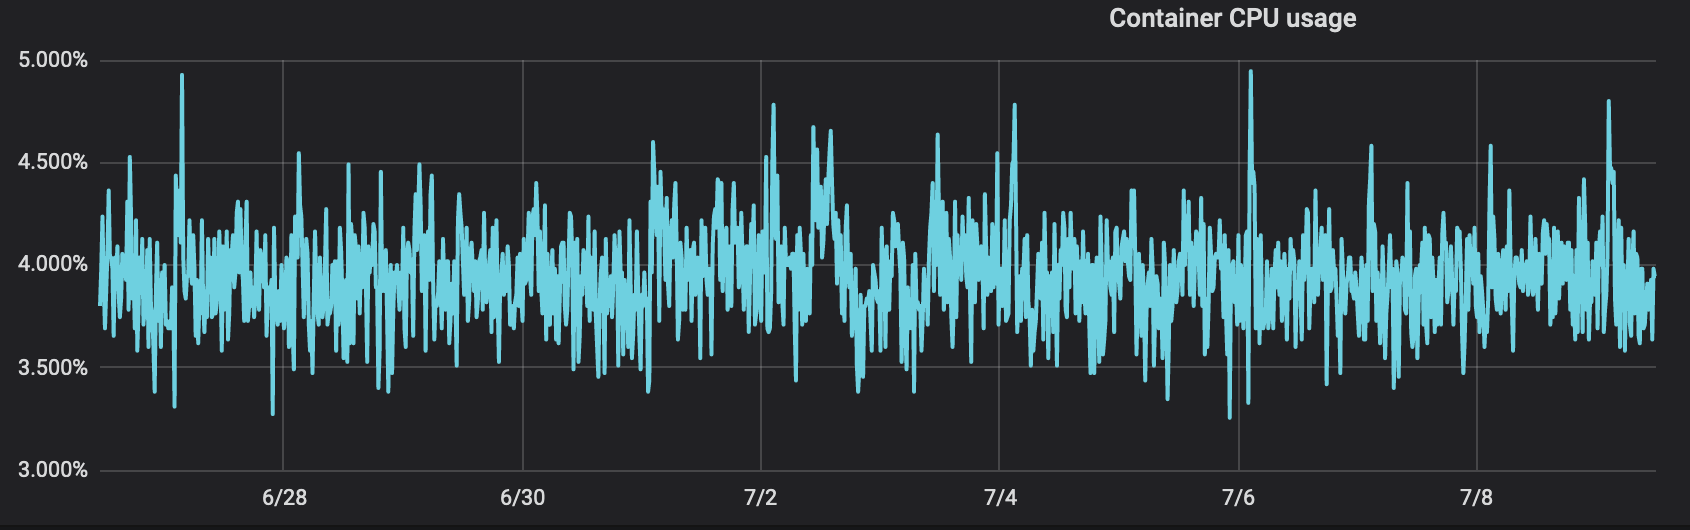
\includegraphics[width=0.45\textwidth]{gfx/vanaheim.png}
        \label{fig:deployment:vanaheim}
    }\qquad
    \subfloat[Host $2$]{
        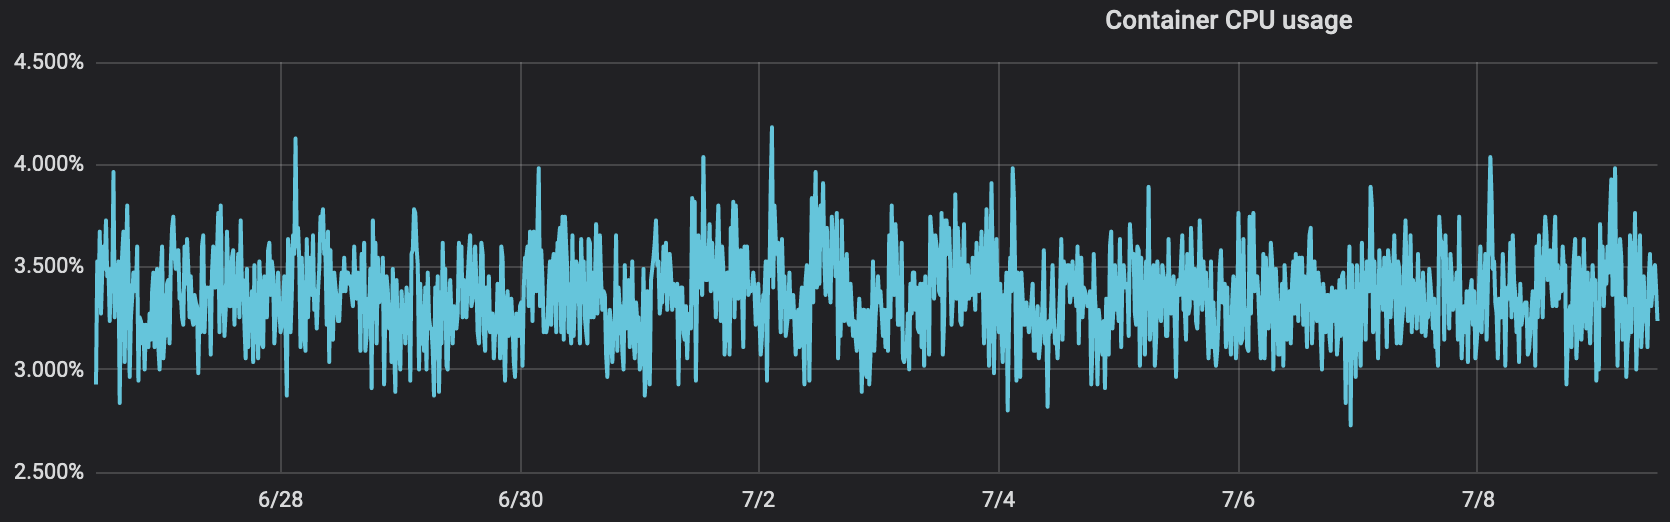
\includegraphics[width=0.45\textwidth]{gfx/alfheim.png}%
        \label{fig:deployment:alfheim}
    }
    
    \subfloat[Host $0$]{%
        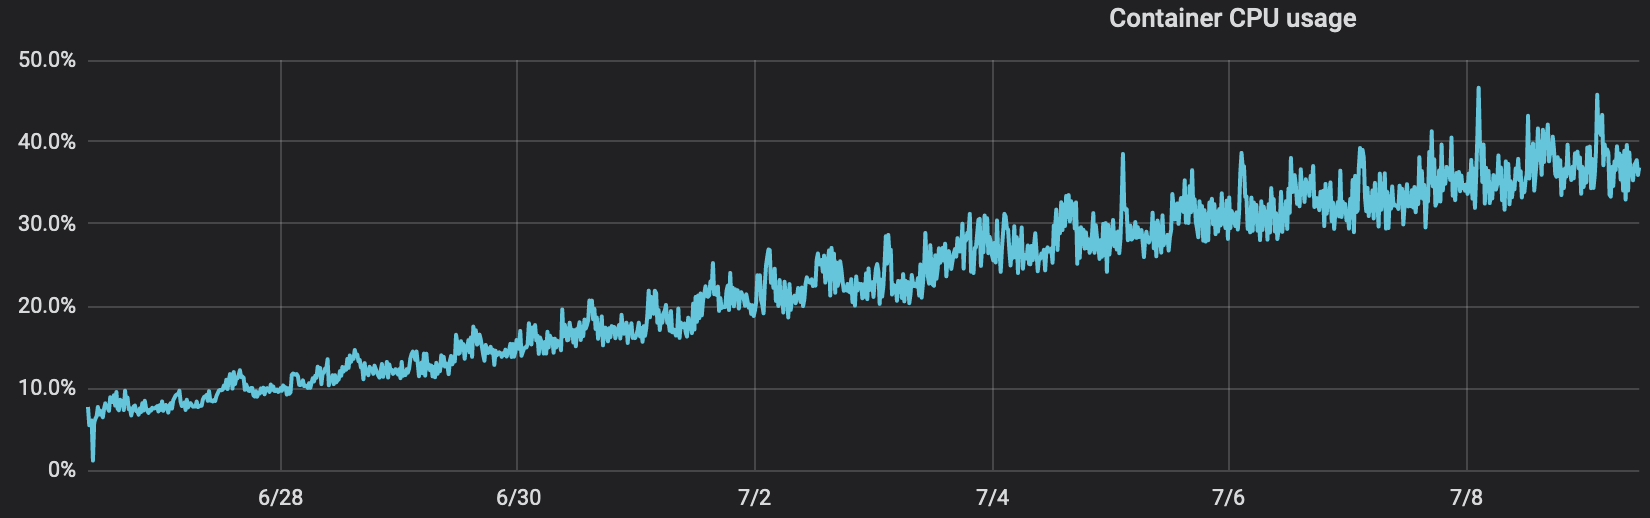
\includegraphics[width=0.45\textwidth]{gfx/jotunheim.png}
        \label{fig:deployment:jotunheim}
    }\qquad
    \subfloat[Host $5$]{
        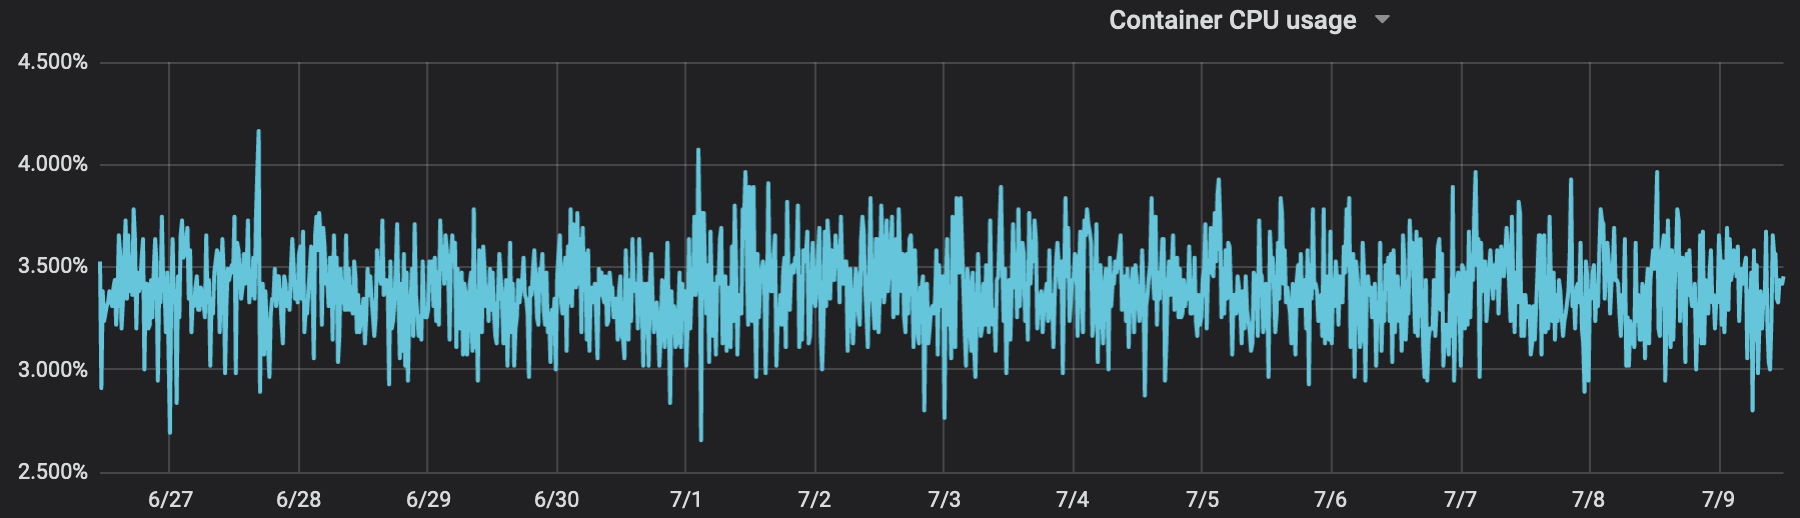
\includegraphics[width=0.45\textwidth]{gfx/niflheim.png}%
        \label{fig:deployment:niflheim}
    }
    
    \subfloat[Root: Host $0$]{%
        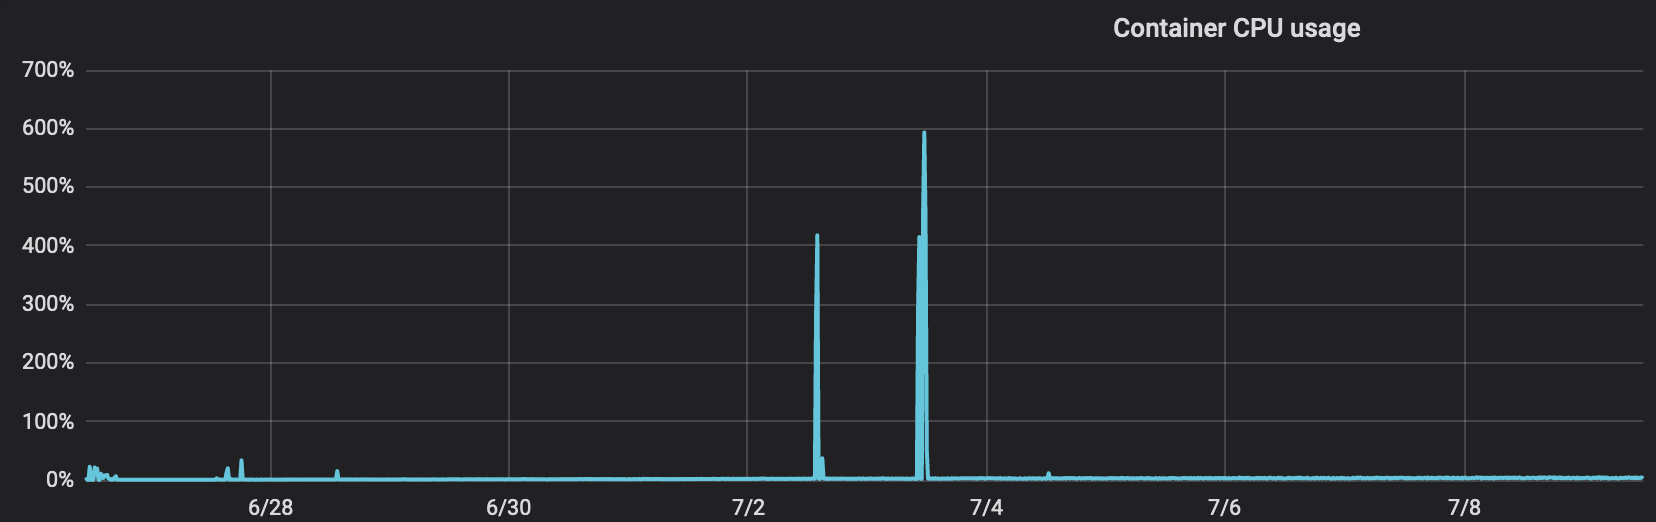
\includegraphics[width=0.45\textwidth]{gfx/jotunheim-root.png}
        \label{fig:deployment:jotunheim-root}
    }
    \caption{CPU utilization of the deployed system at 6 different VMs.}
    \label{fig:deployment}
\end{figure}

\subsection{Third meeting}
In order to solve the issue from the second meeting, the decision was made to implement a batch processing function. This means that the program resolves the network traffic packets afterwards instead of real-time. The decision was made to resolve the packets during the sleeping period, as mentioned in \autoref{sec:exposing_data}. This leads to a more efficient use of the resources, which can be seen in \autoref{fig:deployment}. This figure shows the CPU usage during the lifetime of the system. It can be concluded that the overall  CPU percentage is low, around 4\% for the nodes. The Root at host $0$ shows an average of 2.5\% CPU.

\section{Results}\label{sec:sb-results}
In order to simply the results, several containers are grouped together using a regular expression as explained in \autoref{sec:aggregating_results}. If a certain container name matches a regular expression, then this container is assigned to a certain group. The `other' group acts as a wildcard, matching every container that does not belong to a group. \autoref{tab:regex} shows the groups that are proposed, as well as the number of containers in this group.\\

\begin{table}[H]
    \centering
    \begin{tabular}{l|lr}
        Regular expression & Group name & Containers \\ \hline
        / & other & $42$ \\
        spark & sparkthings & $5$\\
        flink & flinkthings & $4$\\
        zookeeper & zookeeper & $5$\\
        kafka & kafka & $11$\\
        exporter & node-exporter & $5$\\
        socat & socats & $6$\\
        cassandra & cassandra & $3$\\
        rest & timeseriest-rest & $3$\\
        vault & vault & $6$\\
        hadoop & hadoop & $4$\\
        airflow & airflow & $3$\\
        orchestrator & orchestrator & $2$\\
        mw & middlewares & $12$\\
    \end{tabular}
    \caption{Assigning container groups}
    \label{tab:regex}
\end{table}

\begin{table}
    \centering
    \begin{tabular}{l|rrr}
        Group name & CPU usage (cores) & Memory usage & Cost \\ \hline
        other       & $1.8$     & $9$ GB & $\$0.10$ \\
        sparkthings & $0.0066$  & $1$ GB & $<\$0.01$\\
        flinkthings & $2.0$     & $9$ GB & $\$0.07$ \\
        zookeeper   & $0.0085$ &$775$ MB & $<\$0.01$\\
        kafka       & $10.3$    & $6$ GB & $\$0.24$ \\
        node-exporter & $0.014$ &$66$ MB & $<\$0.01$\\
        socats      & $0.00059$ & $5$ MB & $<\$0.01$\\
        cassandra   & $0.70$   & $16$ GB & $\$0.06$ \\
        timeseriest-rest&$0.19$ & $3$ GB & $\$0.01$ \\
        vault       & $0.011$ & $636$ MB & $<\$0.01$\\
        hadoop      & $0.011$ & $342$ MB & $<\$0.01$\\
        airflow     & $0.44$  & $552$ MB & $\$0.01$ \\
        orchestrator& $0.019$ & $371$ MB & $<\$0.01$\\
        middlewares & $0.24$    & $5$ GB & $\$0.02$ \\
    \end{tabular}
    \caption{Cost results for the Smart Buildings company}
    \label{tab:sb-results-cost}
\end{table}

\begin{table}
    \centering
    \begin{tabular}{l|rrr}
        Group name & CPU waste (cores) & Memory waste & Waste cost \\ \hline
        other       & $6.3$ &   $7$ GB & $\$0.16$ \\
        sparkthings & $1.2$ & $955$ MB & $\$0.03$ \\
        flinkthings & $0.21$&  $54$ MB & $<\$0.01$ \\
        zookeeper   & $1.2$ & $978$ MB & $\$0.03$ \\
        kafka       & $1.8$ &   $1$ GB & $\$0.04$ \\
        node-exporter& $1.2$&   $1$ GB & $\$0.03$ \\
        socats      & $1.4$ &   $2$ GB & $\$0.04$ \\
        cassandra   & $0.44$&    $0$ B & $\$0.01$ \\
        timeseriest-rest&$0.72$&$306$ MB &$\$0.02$ \\
        vault       & $1.5$ &   $2$ GB & $\$0.04$ \\
        hadoop      & $0.99$&   $1$ GB & $\$0.03$ \\
        airflow     & $0.40$& $714$ MB & $\$0.01$ \\
        orchestrator& $0.43$& $421$ MB & $\$0.01$ \\
        middlewares & $1.9$ & $750$ MB & $\$0.04$ \\
    \end{tabular}
    \caption{Waste cost results for the Smart Buildings company}
    \label{tab:sb-results-waste}
\end{table}

\noindent
The services at the Smart Buildings Company have been monitored for exactly $14$ days (from June $26$, $11$ AM UTC until July $10$, $11$ AM UTC). During these days, the resources have been monitored on a containerized level, and the waste cost is divided over the running containers. Host $5$ was excluded from the results, as there was an error with the communication with the other hosts. The results of the cost and waste computation is summarized in \autoref{tab:sb-results-cost} and \autoref{tab:sb-results-waste} using \autoref{eq:p}. Note that these tables are constructed from a random hour. This hour has been chosen at it is a representative hour (from $10$ AM UTC till $11$ AM UTC at July $10$), and leads to easy interpretable results. At the end of this section, the results are compared to the average percentages (in \autoref{fig:stats_percentage}) to verify the obtained results.\\

\noindent
Several observations are made from \autoref{tab:sb-results-cost}. First of all, there is no relation between the number of containers in a group, and the cost of this group. As fitting a linear regression in this data results in a precision of $R^2 = 0.16$. The cost of a group and the amount of containers in a group is shown in \autoref{fig:linear-regression}. The second observation that can be made, is that the `kafka' group is the most expensive with $\$ 0.24$ per hour. In general, the costs of a group per hour is quite low, and there are only four groups with a price of more than $\$0.05$ per hour. These groups are: `other', `flinkthings', `kafka' and `socats'. The total amount of effective cost per hour is $\$0.51$\footnote{The cost of a group with $<\$0.01$ is interpreted as $\$0.00$.}.\\

\noindent
The same observations can also be made from \autoref{tab:sb-results-waste}. Using this table, we find a relation between the waste and the number of containers in a group. This is presented in \autoref{fig:linear-regression}. The waste costs are presented in red. The linear regression is shown in a red line. The X-axis presents the number of contains, and the Y-axis presents the waste cost. Using a linear regression, we obtain that the waste cost can be computed estimated using the formula: $C_\text{waste} = 0.0038*n + 0.002$, where $n$ is the number of containers. This formula fits with a precision of $R^2 = 0.94$. Another observation is that the `other' group is responsible for $\$0.16$ waste cost. All other groups are below a waste cost of $0.05$. The only group that does not fit well in this model is `flinkthings'. This is due to the four containers, which all consume more resources than an average container in the industrial company. The total waste cost per hour is $\$0.49$.\\


\begin{figure}
    \centering
    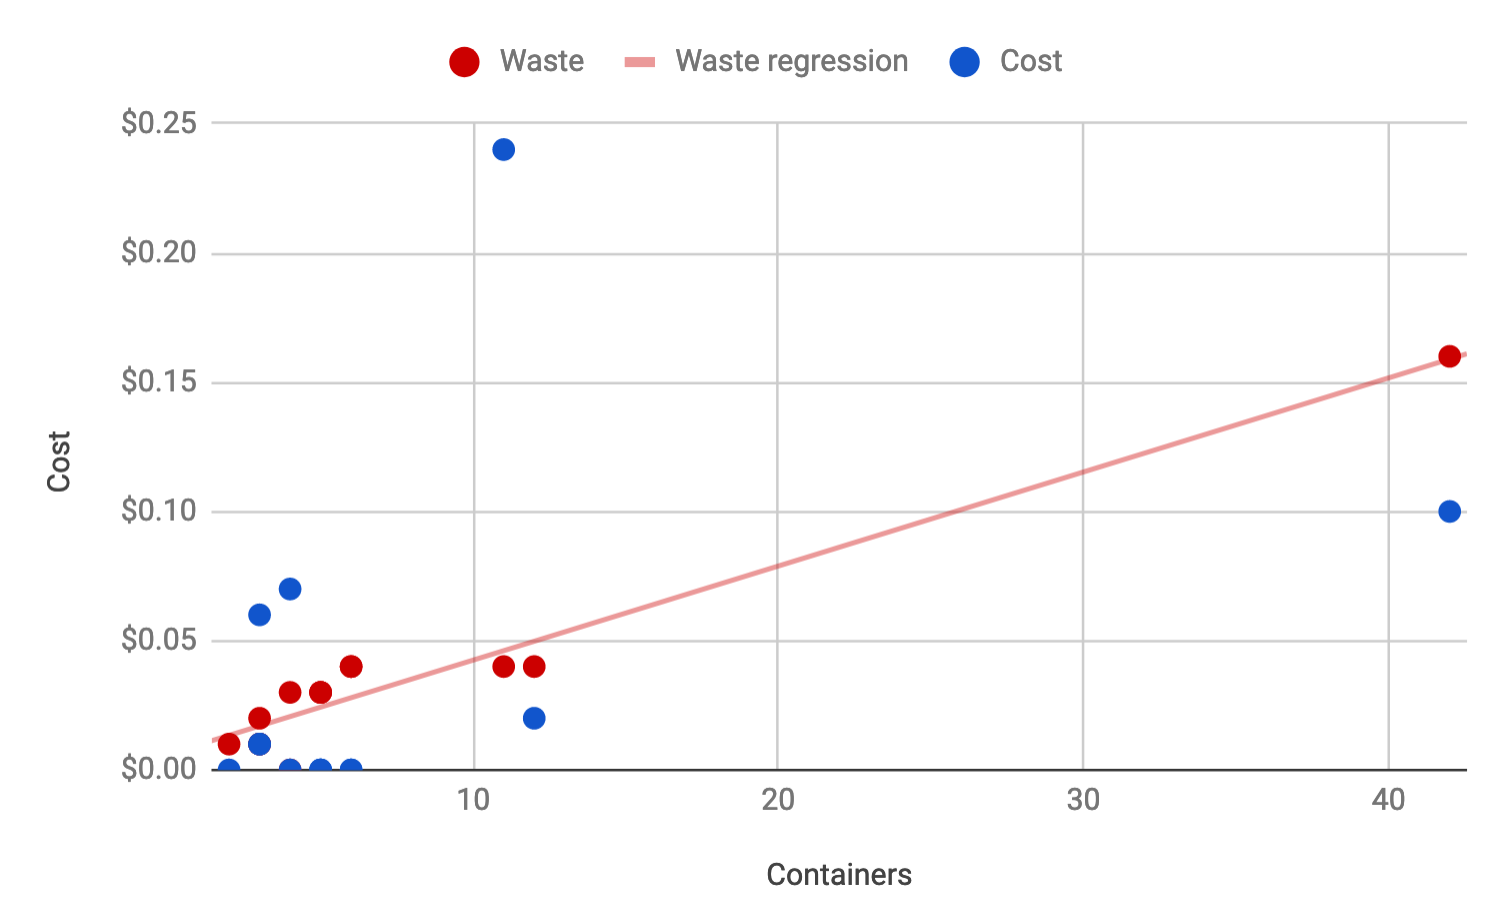
\includegraphics[width=\textwidth]{gfx/linear-regression.png}
    \caption{Relation between the waste cost and the number of containers}
    \label{fig:linear-regression}
\end{figure}

\noindent
The totals shown in \autoref{fig:stats} are the running total cost during the entire monitoring period (i.e. 14 days). They roughly correspond to the values in the two tables above, as a waste cost of $\$0.49$ per hour results in the $\$164.64$ over a time of two weeks. This is equivalent to the total waste cost of $\$160.06$\footnote{This is the sum of \textit{the CPU waste cost} and \textit{the memory waste cost}.}. Secondly, the effective cost of $\$0.51$ per hour is $\$171.36$ over two weeks. This is roughly the same as $\$174.57$\footnote{This is the sum of the \textit{effective CPU cost} and \textit{the effective memory cost}.}. Therefore, we can conclude that the randomly picked hour is representative for the overall resource utilization of the company.


\noindent
The total effective cost per hour ($\$0.51$) and the total waste cost per hour ($\$0.49$) as discussed in the previous two paragraphs can be used for computing the waste ratio, which is $49\%$. However, this is higher than the average during the monitoring period, which can be seen in \autoref{fig:stats_percentage}. This is due to the fact that the company runs a number of batch jobs during the night. Therefore, the resources are more consumed during the night, leading to a drop in the overall waste ratio. \autoref{sec:sb-limitation} describes the limitations with respect to the network traffic monitoring, resulting in an adjusted network price of $p_\text{network} = 0.05$. This is half of the proposed pricing. This is based on the assumption that half of the network traffic is internal (between their services), and other half of the network traffic is external. Lastly, the total CPU cores used is $15.74$ and the total CPU cores unused is $19.69$. This results in a CPU waste ratio of $44.4\%$. This value is lower than the ratio in \autoref{fig:stats_percentage}, due to the mentioned reason above. The total memory used is $50.7$ GB and the total memory unused is $18.1$ GB. The memory waste ratio is therefore $26.3\%$, this is similar to the presented result in \autoref{fig:stats_percentage}.\\

\begin{figure}
    \centering
    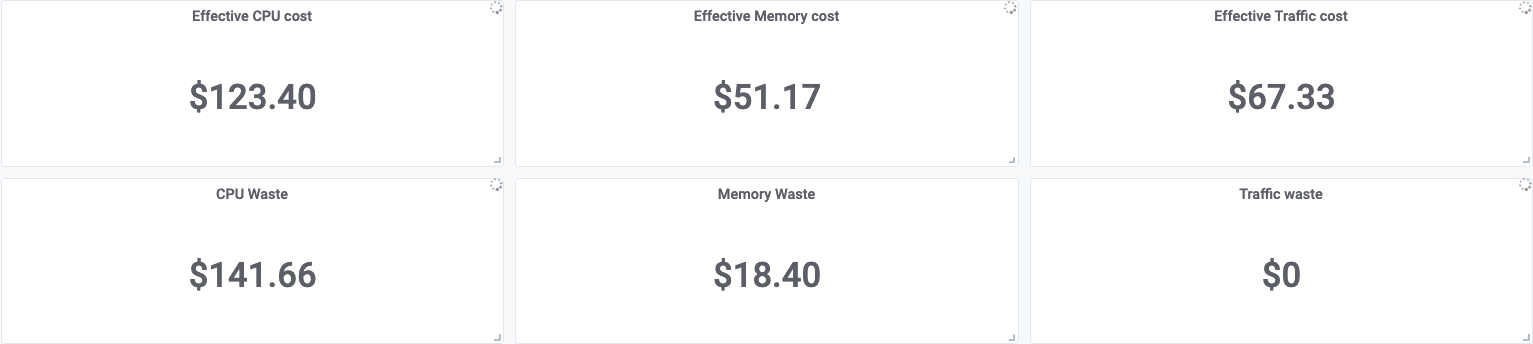
\includegraphics[width=\textwidth]{gfx/stats.png}
    \caption{Overall stats of the Smart Buildings Company}
    \label{fig:stats}
\end{figure}

\begin{figure}
    \centering
    
\includegraphics[width=\textwidth]{gfx/stats_percentage.png}
    \caption{Percentage stats of the Smart Buildings Company}
    \label{fig:stats_percentage}
\end{figure}

\label{sec:sb-limitation}
\noindent
The system proposed in \autoref{ch:design} is able to monitor the CPU and memory usage on a containerized level. Using TCPdump, a subsampling procedure is implemented that monitors the packets on a host level. Then, the system assigns this packets to a container by resolving their IP address. However, almost all the communication in the industrial company are configured using Weave Net\footnote{See \url{https://github.com/weaveworks/weave}}. Weave Net creates a virtual network that connects Docker containers across multiple hosts and enables their automatic discovery. To application containers, the network established by Weave resembles a giant Ethernet switch, where all containers are connected and can easily access services from one another. \cite{weave}.\\

\noindent
When using the weave network, the containers do not communicate by their exposed IP address. Therefore, the proposed system is unable to resolve the network packets. This leads to a lower estimate of $n_\text{internal}$ in \autoref{formula:traffic}, which results in a higher $n_\text{network}$. Therefore, the estimated cost using \autoref{eq:p} is also too high. Further work is needed to resolve the IP addresses according to the weave network.


\section{Interview} \label{sec:sb-interview}
In order to evaluate the deployment process of the system, we decided to interview a technical employee at the company, as he contributed in deploying the monitoring solution. The entire interview can be found in \autoref{ch:interview}. The interview is divided into questions about the process and about the final delivered work.\\

\noindent
The process consists of multiple sprints with a duration of one week. During a sprint, the problems are fixed that arise in the previous sprint. The answer in $Q2$ concludes that the quality of the deployed solution has improved over the sprints, resulting in a more general solution, due to the configurability of the solution.\\

\noindent
The final delivered work is considered of a good overall quality, as can be concluded from $Q4$. Furthermore, the cost model that is implemented in the proposed solution shows a high accuracy rate. In the answer of $Q5$, the limitations of the solution are confirmed as well. A remark that the technical employee makes is with respect to the waste estimation in $Q5$: ``A high waste does not necessarily imply that this can be optimized, as the VM's have peak loads which require the overhead which lead to waste when there is no peak.'' The last question ($Q9$) confirms that the technical employee is satisfied with the proposed solution, and will be used in the future for a longer amount of time.

\section{Conclusion} \label{sec:sb-evaluation}
From the case study, several observations can be made. First of all, the quality of the implemented solution was substandard during the first and second meeting. Due to the made improvements, it can be concluded that the quality has improved, leading to quality-level that is sufficient for production use. However, there are still improvements to be made, due to the issue described in \autoref{sec:sb-limitation}. The cost model is of a high accuracy, as confirmed in \autoref{sec:sb-interview}. Lastly, the technical employee argues to be happy with the solution, and will be used in the future.\\

\noindent
For the reproducibility of the case study, the data has been made publicly available\footnote{The data can be downloaded from \url{https://drive.google.com/file/d/1SUy_j3WpSjCaZ54KeotaE4xhF87rrjwh/view?usp=sharing}}. This file is the compressed data folder from the Prometheus database. This can therefore be used to generate the visualizations above.